\documentclass[11pt]{article}
\usepackage[T1]{fontenc}
\usepackage[margin=1in]{geometry}
\usepackage{amsmath,amssymb}
\usepackage{graphicx}
\usepackage{booktabs}
\usepackage{longtable}
\usepackage{array}
\usepackage{xcolor}
\usepackage[colorlinks=true,linkcolor=blue!60!black,urlcolor=blue!60!black,
            citecolor=blue!60!black]{hyperref}
\usepackage[htt]{hyphenat}
\usepackage{microtype}
\emergencystretch=3em
\usepackage{listings}
\lstset{basicstyle=\ttfamily\footnotesize, backgroundcolor=\color{gray!8},
        frame=single, rulecolor=\color{gray!40}, breaklines=true,
        columns=fullflexible, keepspaces=true, showstringspaces=false}

\newcommand{\code}[1]{\texttt{#1}}
\newcommand{\file}[1]{\texttt{\small #1}}
\newcommand{\St}{S}
\newcommand{\ts}{t_{\rm s}}
\newcommand{\vf}{v_{\rm frag}}
\newcommand{\pass}{\textcolor{green!45!black}{\textbf{PASS}}}

\title{Dust Growth on Superparticles in AthenaK\\[0.4em]
       \large \textsc{Validation Document}\\
       \large D3 tests (a)--(e), cost, and R1: the stratified SI with growth}
\author{worktree \code{athenak-worktrees/dust-growth}, branch \code{dust-growth}
        (parent \code{9aaa5639})\\
        \small commits \code{a821cb4d} (growth step, diagnostics, tests) and
        \code{e231fc7f} (\code{nsh\_init}, R1 set-up)}
\date{October 19--20, 2026}

\begin{document}
\maketitle

\begin{abstract}
\noindent
Five tests of the per-superparticle growth step described in
\file{dust\_growth\_implementation.pdf}, all passing: (a) with growth off the code is
byte-identical to its parent; (b) uniform growth follows the analytic $\St(t)$ with
first-order convergence in $\Delta t$; (c) fragmentation holds the turbulent cap
$\St_{\rm frag}=\vf^2/(3\alpha_t c_s^2)$ to 0.2\%; (d) the drift term reproduces the
Nakagawa--Sekiya--Hayashi relative velocities of three species to $10^{-12}$ in 2D,
in 3D with orbital advection and in 3D without; (e) the stopping times survive a
restart bitwise and pass through AMR particle splitting unchanged. The growth step
costs 1--8\% per cycle. R1, the stratified streaming instability in a thin 3D box at
$1280/H$ with $Z=0.02$, $\Pi=0.05$ and grains starting at $\St=10^{-3}$ (below the
clumping threshold), shows the effect growth has: the grains reach the fragmentation
cap $\St\approx0.33$ within $\sim\!55\,\Omega^{-1}$, and the particle density exceeds
the Hill density from $t=82\,\Omega^{-1}$ to the end of the run ($300\,\Omega^{-1}$,
peak $1920\rho_{g0}$), while the identical run without growth never exceeds
$2.9\rho_{g0}$.
\end{abstract}

\tableofcontents

%=========================================================================================
\section{Summary}

\begin{longtable}{>{\raggedright\arraybackslash}p{0.25\linewidth}>{\raggedright\arraybackslash}p{0.53\linewidth}p{0.12\linewidth}}
\toprule
test & result & status \\
\midrule
{}(a) growth off & all data outputs byte-identical to the parent (2D NSH, 3D AMR on 4
  ranks, YJ14 stratified on 4 ranks) & \pass \\
{}(b) uniform growth & error $2.8\times10^{-3}$ at $C=0.45$, halving with $\Delta t$
  (order 0.998, 0.999) & \pass \\
{}(c) fragmentation cap & $\St$ held within $-0.22\%$ / $+0.12\%$ of $\St_{\rm frag}$;
  reached at $t=8.76$ (law: 8.74) & \pass \\
{}(d) drift vs NSH & three species, three geometries: relative error $\le1.2\times10^{-12}$
  & \pass \\
{}(e) restart, AMR & restart bitwise; AMR run with splitting completes on 4 ranks;
  split keeps $\max\St$, $\min\St$ bitwise & \pass \\
\bottomrule
\end{longtable}

\subsection{Reproducing}
From the repository root of the worktree, with the new binary in \file{build/src/athena}
and a baseline binary of the parent commit (default: the \code{si-strat-amr} worktree's
build, which is at \code{9aaa5639}):
\begin{lstlisting}
scripts/analysis/dust_growth_tests.sh all        # runs -> validation/run/dust_growth/
python3 scripts/analysis/dust_growth_tests.py    # checks; PASS/FAIL per test
julia scripts/analysis/dust_growth_tests_fig.jl  # validation/figures/dust_growth_tests.png
\end{lstlisting}
The suite takes about 5 minutes on 4 Mac cores. AthenaK's command line can only replace
parameters that already exist in an input file (new parameters or blocks are a fatal
error), so the shell script writes a patched copy of the input into every run directory
(\code{patch\_input}).

%=========================================================================================
\section{Test (a): growth off is the parent code}

\paragraph{Purpose.} The growth task is added to every dust run; with
\code{growth = none} it must change nothing.

\paragraph{Set-up.} The parent binary and the new binary run three existing inputs with
identical patched copies:
\begin{itemize}
\item \file{dust\_nsh.athinput}: 2D $r$--$z$ shearing box, three species, NSH
  equilibrium, to $t=2$ (1 rank);
\item \file{dust\_nsh\_shear3d\_amr.athinput}: 3D shear-periodic NSH with an AMR refine
  and derefine event and particle splitting, one orbit (4 ranks);
\item \file{streaming\_strat\_yj14.athinput}: 3D stratified SI, WENO-Z + Roe,
  60 cycles with every output (hst, phst, dust density and gas VTK, float64 particle VTK,
  restart) written frequently (4 ranks).
\end{itemize}

\paragraph{Result.} Every data file is byte-identical: 4/4, 4/4 and 23/23 files. The two
restart files of the YJ14 case differ only in their parameter block, where the new
binary echoes the defaulted line \code{growth = none \# Default value added at run time}
(76 bytes); the binary payload after \code{<par\_end>} is identical. After the
\code{nsh\_init} option was added to \code{streaming\_strat}, the YJ14 comparison was
repeated (20/20 data files identical), confirming that the generator is unchanged with
the option off.

%=========================================================================================
\section{Test (b): uniform growth}

\paragraph{Set-up.} \file{inputs/dust/dust\_growth\_box.athinput}: 2D $r$--$z$ shearing
box, $32^2$ cells, $L=1\,H$, periodic, one species on the quiet lattice of the
\code{dust\_nsh} generator (1 particle per cell), $\epsilon=\rho_d/\rho_{g0}=1$, no
pressure gradient ($\eta=0$) and no back-reaction. Gas and dust stay exactly at rest,
so the drift term is zero, and the lattice makes the TSC density exactly 1 at every
particle. $\St_0=10^{-3}$, $\alpha_t=10^{-3}$, $\vf=10\,c_s$ (no fragmentation),
$t_{\rm end}=20\,\Omega^{-1}$.

\paragraph{Expected.} With $\Delta v=\sqrt{3\alpha_t\St}c_s$, the law
$d\St/dt=\sqrt{\pi/8}\,\Omega\,(\rho_d/\rho_{g0})\,\Delta v/c_s$ becomes
$d\sqrt{\St}/dt=\tfrac12\sqrt{\pi/8}\,(\rho_d/\rho_{g0})\sqrt{3\alpha_t}\,\Omega$, so
\begin{equation}
  \St(t)=\Bigl[\sqrt{\St_0}+\tfrac12\sqrt{\pi/8}\,\tfrac{\rho_d}{\rho_{g0}}
         \sqrt{3\alpha_t}\,\Omega t\Bigr]^2 ,
  \qquad \St(20)=0.140518 .
\end{equation}
The forward-Euler split is first order, so the error should halve with $\Delta t$.

\paragraph{Result.} Three Courant numbers (Fig.~\ref{fig:tests}, first two panels):
\begin{center}
\begin{tabular}{cccc}
\toprule
$C$ & $\St(t=20)$ & max $|\St/\St_{\rm exact}-1|$ & order \\
\midrule
0.45 & 0.140294 & $2.801\times10^{-3}$ & \\
0.225 & 0.140406 & $1.402\times10^{-3}$ & 0.998 \\
0.1125 & 0.140462 & $7.014\times10^{-4}$ & 0.999 \\
\bottomrule
\end{tabular}
\end{center}
All particles keep identical $\St$ (spread 0). The error peaks early, when
$d\ln\St/dt$ is largest, and the per-cycle cap (5\%) never binds. In production the
per-step change is $\sim\Delta t/t_{\rm grow}\sim10^{-5}$, so the splitting error is
negligible there.

\begin{figure}[t]
\centering
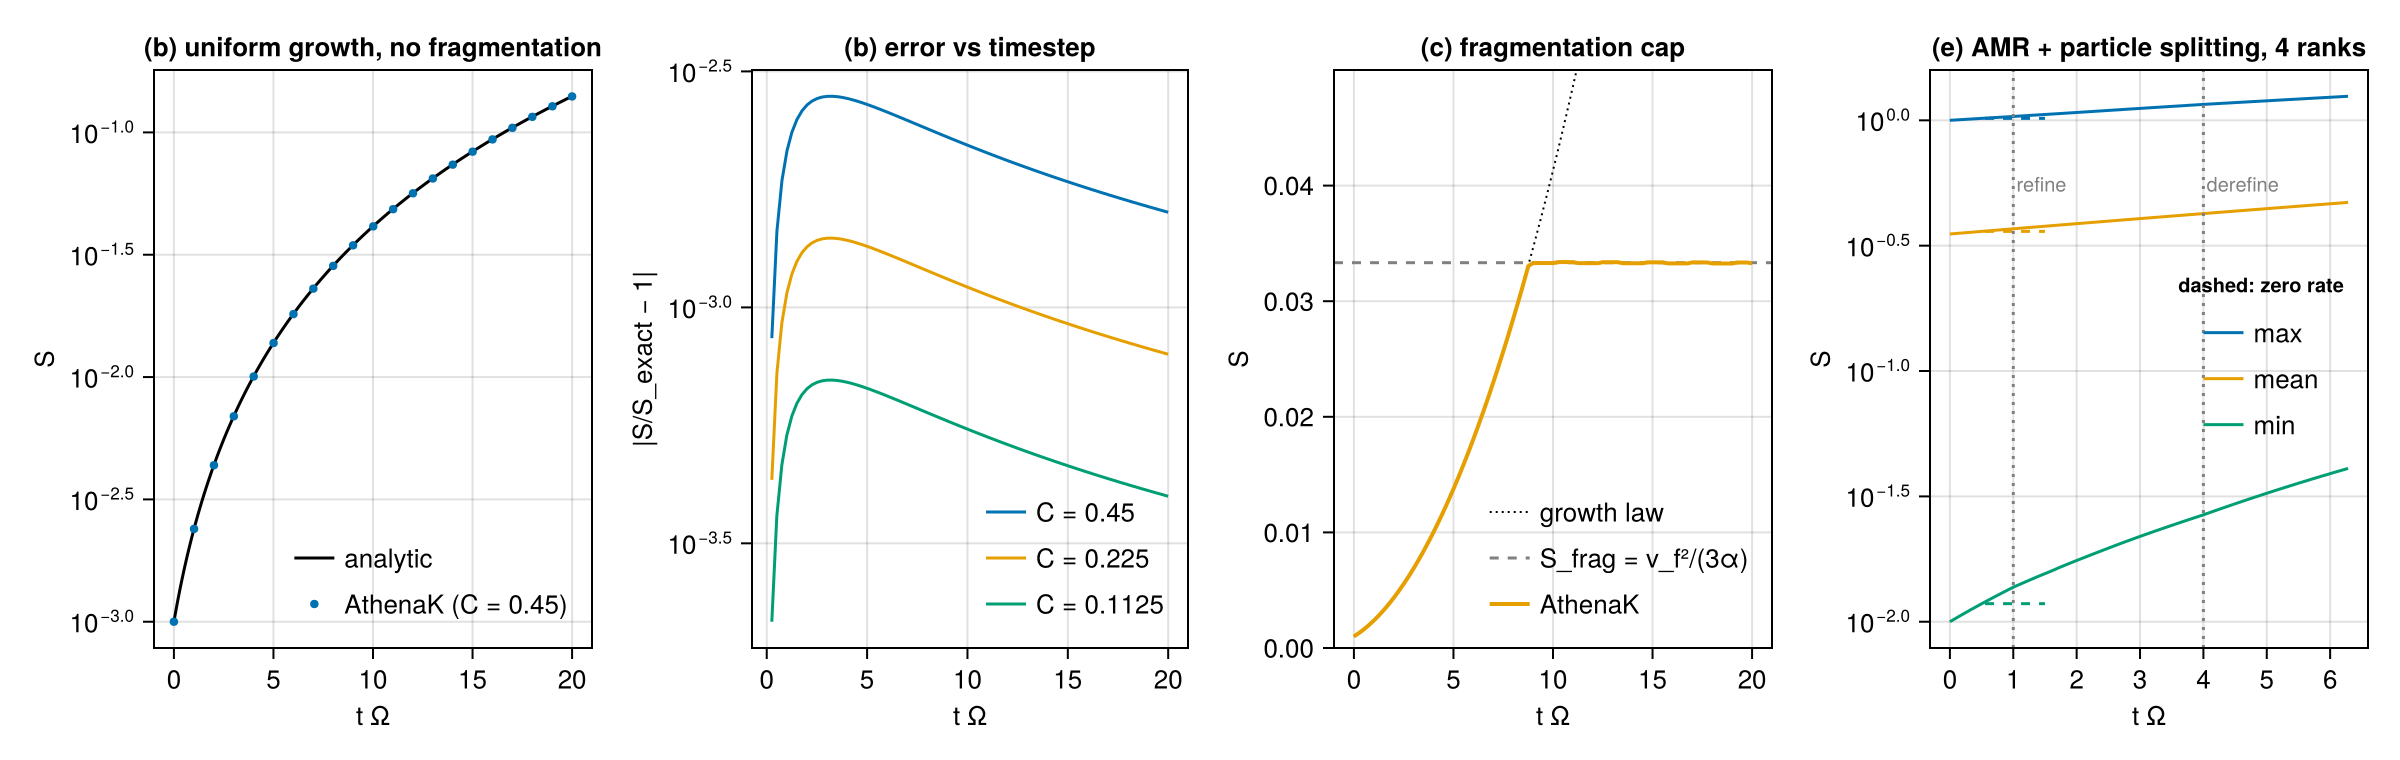
\includegraphics[width=\linewidth]{figures/dust_growth_tests.png}
\caption{(b) Mass-weighted mean Stokes number against the analytic law, and its error
at three Courant numbers. (c) With $\vf=0.01c_s$ the growth stops at
$\St_{\rm frag}=0.0333$. (e) The 3D AMR NSH run with growth on 4 ranks (solid: max,
mass-weighted mean, min of $\St$; dotted lines: the refine and derefine events); dashed:
the restart at $t\approx0.55$ with a zero growth rate, flat through the split at
$t\approx1.05$.}
\label{fig:tests}
\end{figure}

%=========================================================================================
\section{Test (c): the fragmentation cap}

\paragraph{Set-up.} As (b) with $\vf=0.01c_s$, so the turbulent cap is
$\St_{\rm frag}=\vf^2/(3\alpha_tc_s^2)=0.0333$.

\paragraph{Result.} $\St$ follows the growth law until $t=8.76$ (the law reaches
$0.99\St_{\rm frag}$ at 8.74), then dithers at the cap: for $t>12$ the mass-weighted
mean lies in $[0.033260, 0.033375]$, i.e.\ $-0.22\%$ to $+0.12\%$ of $\St_{\rm frag}$,
and the overall maximum is 0.033384. The dither amplitude is one step's change at the
cap, as designed (Fig.~\ref{fig:tests}, third panel).

%=========================================================================================
\section{Test (d): the drift term against NSH}

\paragraph{Set-up.} \file{dust\_nsh.athinput} (2D $r$--$z$, 1 rank) and
\file{dust\_nsh\_shear3d.athinput} (3D shear-periodic, 4 ranks, with and without
orbital advection), growth on with $\alpha_t=0$ (drift only) and $\vf=10c_s$, one cycle,
float64 particle VTK at cycles 0 and 1. Three species with $\tau_s=0.01, 0.1, 1$ and
$\epsilon_s=0.2, 0.5, 0.3$, $\eta v_K=0.05c_s$, $q=3/2$, lattice placement at the exact
multi-species NSH equilibrium.

\paragraph{Expected.} Over the first cycle each particle's $\ts$ changes by
$\Delta t\,\sqrt{\pi/8}\,(\rho_d/\rho_{g0})\,\tfrac12|\mathbf v_s-\mathbf u|/c_s$ with
$\rho_d=\sum_s\epsilon_s\rho_{g0}=1$ and $|\mathbf v_s-\mathbf u|$ from the
multi-species NSH linear system, solved independently in the checker
(\file{dust\_growth\_tests.py}, \code{nsh\_dv}).

\paragraph{Result.} Measured $(\ts^{(1)}-\ts^{(0)})/\Delta t$, mean over each species,
with the largest relative deviation of any particle:
\begin{center}
\begin{tabular}{lccc}
\toprule
geometry & species 1 & species 2 & species 3 \\
\midrule
2D $r$--$z$ & $1.6819390297\times10^{-4}$ & $1.6797615195\times10^{-3}$ &
  $1.0029805021\times10^{-2}$ \\
 & ($2.3\times10^{-13}$) & ($3.2\times10^{-14}$) & ($7.2\times10^{-13}$) \\
3D, FARGO & same digits & same digits & same digits \\
 & ($3.0\times10^{-13}$) & ($7.7\times10^{-14}$) & ($3.7\times10^{-13}$) \\
3D, no FARGO & same digits & same digits & same digits \\
 & ($5.2\times10^{-14}$) & ($8.9\times10^{-14}$) & ($1.2\times10^{-12}$) \\
\midrule
expected & $1.6819390297\times10^{-4}$ & $1.6797615195\times10^{-3}$ &
  $1.0029805021\times10^{-2}$ \\
\bottomrule
\end{tabular}
\end{center}
This checks the gather of the gas velocity, the pairing of velocity components in the
2D $r$--$z$ box (azimuthal = third component), and, in the no-FARGO case, the
background-shear correction applied at the stencil cells, which is exact because TSC
weights reproduce linear functions.

%=========================================================================================
\section{Test (e): restart and AMR}

\subsection{Restart}
\paragraph{Set-up.} The test box with drift ($\eta v_K=0.05c_s$, back-reaction on,
$\alpha_t=10^{-3}$), run to $t=4$ writing a restart file at $t\approx2$; a second run
restarts from that file and continues to $t=4$. (A first version restarted from a run
stopped at $t_{\rm lim}=2$; its shortened last step changes the timestep sequence, so
that comparison is not bitwise by construction.)
\paragraph{Result.} The final float64 particle VTK files of the straight and restarted
runs are byte-identical.

\subsection{AMR and particle splitting}
\paragraph{Set-up.} \file{dust\_nsh\_shear3d\_amr.athinput} with growth
($\alpha_t=10^{-3}$, drift on): the interior bar refines at $t=1$ (every particle of a
refining block becomes 8 children) and derefines at $t=4$; 4 ranks; restart file at
$t\approx0.55$. \emph{Split check}: restart from that file with
$\alpha_t=0$ and the drift term off, so the growth rate is exactly zero, and run through
the refine event to $t=1.5$. By $t=0.55$ every $\ts$ has grown away from its species
value, so a split that reset \code{IPTS} to the species table, or lost it, would show.
\paragraph{Result.} The AMR run completes (98\,304 $\to$ 270\,336 particles,
$\langle\St\rangle$ 0.352 $\to$ 0.471). In the split check $\max\St$ and $\min\St$ stay
bitwise constant through the split at $t=1.05$ ($\min\St=0.0118038$ against the species
value 0.01); the mass-weighted columns move by at most $7.7\times10^{-13}$, which is the
round-off of summing 2.75 times as many particles of one eighth the mass.

\paragraph{Not a test: AMR against a uniform mesh.} Comparing this AMR run with a
uniform-mesh twin was the first plan, but the two diverge right after the refine event
whether or not growth is on: refining the NSH lattice makes the particle-mesh deposit
non-uniform (the maximum dust density jumps from 1.000 to 1.09--1.33 while refined, and
to 1.031 after derefinement), and the NSH errors of the unmodified parent at the end of
this input are $10^{-7}$--$10^{-5}$, not the round-off its header claims. This is a
pre-existing property of the AMR lattice test, unrelated to growth, and has been
flagged separately. The same input with \code{<problem>/amr\_test = false} segfaults,
because the generator then enrols no refinement function while the input still asks for
\code{method = user}; the uniform twin was instead run with the refinement window moved
past the end of the run.

%=========================================================================================
\section{Cost}
The growth step adds one particle-mesh deposit, its additive and copy exchanges, and one
pass over the particles per cycle.
\begin{center}
\begin{tabular}{llcc}
\toprule
case & machine & without growth & with growth \\
\midrule
YJ14 box ($32^2\times16$, 16k particles), 300 cycles & Mac, 4 ranks & 1.453 s & 1.466 s
  (+0.9\%) \\
R1 box ($256\times4\times256$, 262k particles) & h-2, 64 ranks & 25.2 s & 27.1 s
  (+7.5\%) \\
 & & \multicolumn{2}{c}{(per 1000 cycles)} \\
\bottomrule
\end{tabular}
\end{center}
The R1 comparison is between the \code{nogrowth} run (\code{species\_fixed}) and the
\code{fid} run (\code{dynamic}), so it also includes the two per-cycle stopping-time
reductions of \code{dynamic} mode.

%=========================================================================================
\section{R1: the stratified SI with growth}

\subsection{Set-up (approved October 19)}
\file{inputs/dust/streaming\_strat\_growth\_r1.athinput}, in the style of Lim et al.\
(2025, ApJ 981, 160) but quasi-2D in a thin 3D box, because the dust module and
\code{streaming\_strat} are 3D-only and the 2D $r$--$z$ shearing box has no vertical
gravity:
\begin{longtable}{>{\raggedright\arraybackslash}p{0.25\linewidth}p{0.68\linewidth}}
\toprule
box & $0.2H\times4\text{ cells}\times0.2H$ at $1280/H$ ($256\times4\times256$), 64
  MeshBlocks of $32\times4\times32$; uniform mesh \\
boundaries & shear-periodic $x$ with orbital advection (FARGO), periodic $y$ and $z$ \\
gas & isothermal, WENO-Z + Roe, $C=0.3$, imex2+ drag \\
dust & $\Pi=0.05$, $Z=0.02$, one species, $\St_0=10^{-3}$, Gaussian layer
  $H_{p0}=0.025H$ with NSH velocities for the local $\epsilon(z)$ (midplane
  $\epsilon=0.80$), 1 particle per cell (262\,144) \\
growth & $\alpha_t=10^{-4}$, $\vf=0.01c_s$ ($\St_{\rm frag}=0.33$), drift on \\
runs & \code{fid} (growth + back-reaction) and \code{nogrowth} ($\St=10^{-3}$ fixed); a
  no-back-reaction control is available (\code{CASE=nobr}) but was not requested \\
machine & h-2, jobs 276 (\code{fid}) and 277 (\code{nogrowth}), 64 ranks each, run
  directories \file{/data/limjay/runs/si\_growth\_r1/\{fid,nogrowth\}}, source
  \file{/data/limjay/athenak\_growth} \\
length & $t=300\,\Omega^{-1}$ ($\approx$48 orbits), $\Delta t=2.2\times10^{-4}$
  ($1.35\times10^6$ cycles); restart files every $100\,\Omega^{-1}$ \\
outputs & hst and phst every $1\,\Omega^{-1}$, dust density every 2, gas every 20,
  particle VTK with \code{ptaus} every 10 \\
\bottomrule
\end{longtable}
Without growth, $\St=10^{-3}$ at $Z=0.02$ lies below the strong-clumping threshold
(Li \& Youdin 2021: $Z_{\rm crit}(10^{-3})\approx0.035$; Lim et al.\ 2025 found no strong
clumping at $\tau_s=0.001$, $Z=0.02$ even at $5120/H$). The question R1 answers is
whether growth carries the system across the threshold.

\subsection{Smoke test at 320/H}
The same input at $320/H$ ($64\times4\times64$, 4 Mac ranks) to $t=60\,\Omega^{-1}$
(Fig.~\ref{fig:smoke}): stable throughout; the mass-weighted mean $\St$ goes
$10^{-3}\to0.017$ ($t=25$) $\to0.17$ ($t=60$); the largest particles reach the cap 0.33
by $t\approx55$; the maximum dust density climbs from 1.5 to 21 as the layer settles and
begins to clump. Particles high in the layer, where $\rho_d$ is small, grow slowly
(minimum $\St$ only 0.002 at $t=60$), so the size distribution is broad. The cap of
5\% per cycle never bound; fragmentation acted on $7.8\times10^6$ particle-steps once
the largest grains reached the cap.

\begin{figure}[t]
\centering
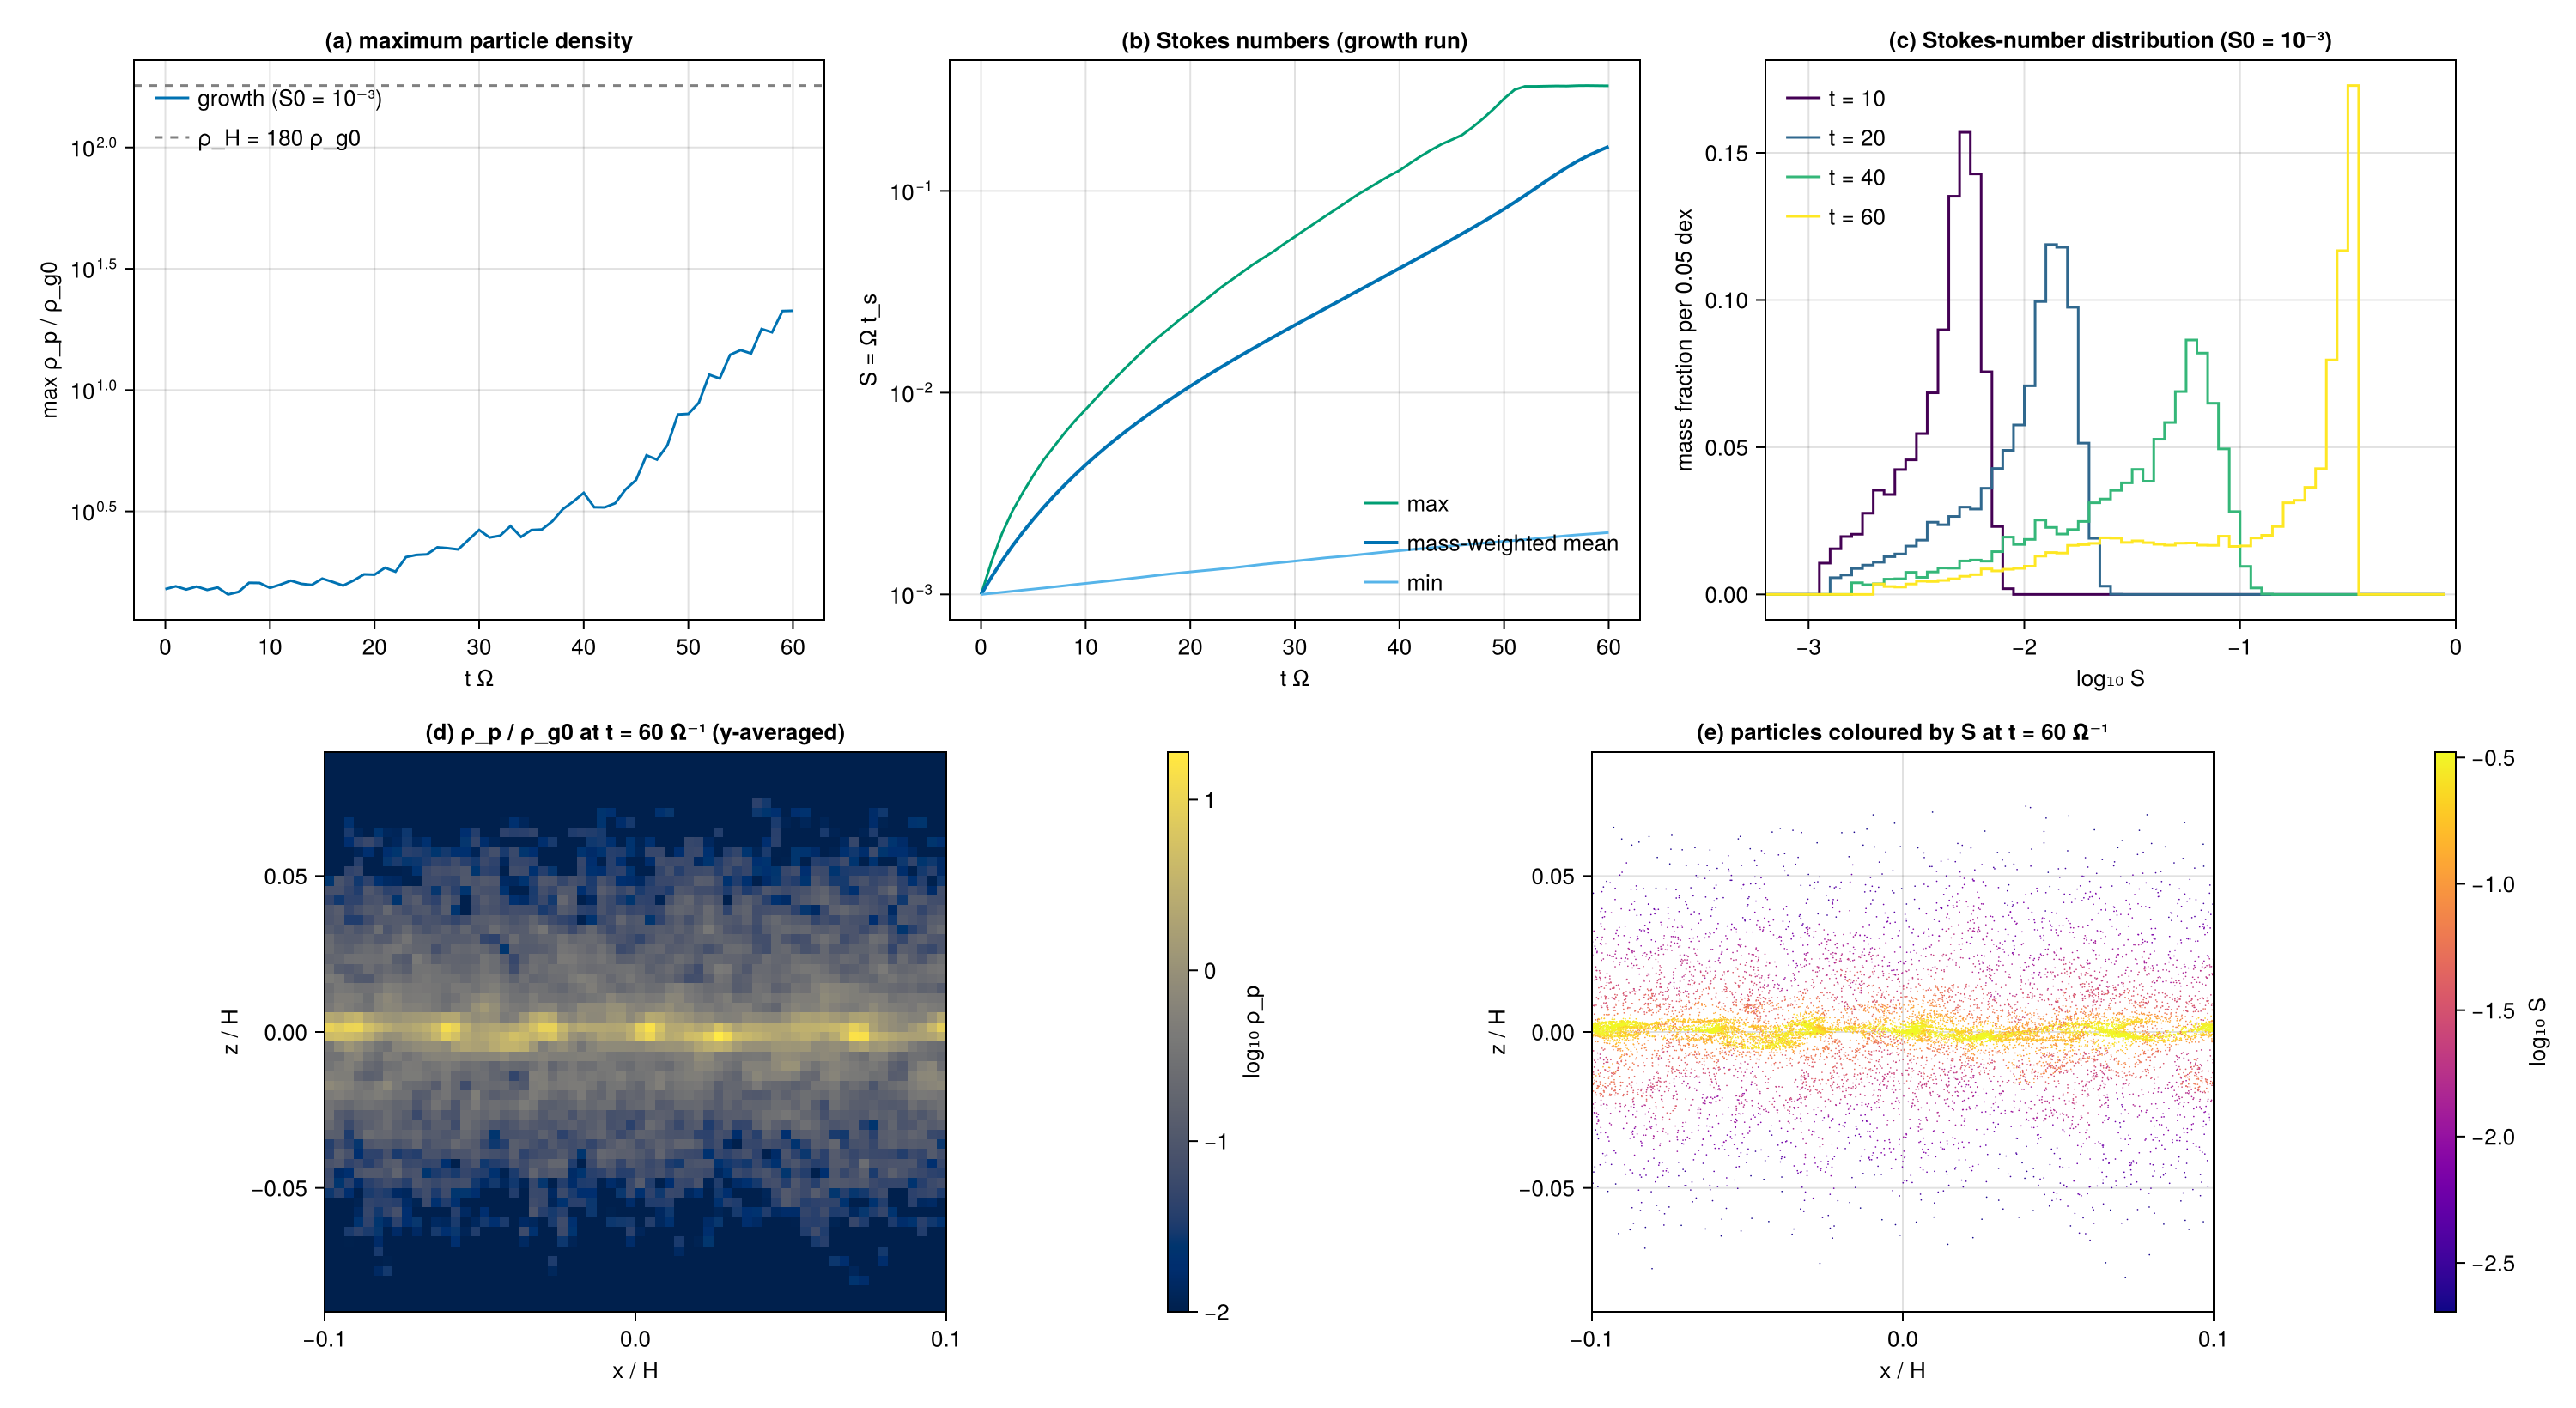
\includegraphics[width=\linewidth]{figures/dust_growth_r1_smoke320.png}
\caption{R1 set-up at $320/H$ (smoke test, growth run only). (a) Maximum dust density
with the Hill density $180\rho_{g0}$ of Lim et al.\ (2025); (b) Stokes-number statistics;
(c) mass distribution of $\St$; (d) $y$-averaged dust density and (e) particles coloured
by $\St$ at $t=60\,\Omega^{-1}$.}
\label{fig:smoke}
\end{figure}

\subsection{Results}
Both runs reached $t=300\,\Omega^{-1}$ (exit 0): \code{nogrowth} in 9.4 h and \code{fid}
in 19.7 h of wall time. \code{fid} started at 27 s per 1000 cycles, like \code{nogrowth}
(25 s), but slowed to 42 s once clumps formed, presumably because the dense regions
load a few ranks heavily (one MeshBlock per rank, uniform mesh). Figure~\ref{fig:r1}
shows the growth run at $t=300$ and both runs' maximum density.

\paragraph{Growth.} The midplane grains grow first, where $\rho_d$ is largest. The
mass-weighted mean Stokes number passes $0.01$ at $t=19$, $0.03$ at $t=35$ and $0.1$
at $t=52\,\Omega^{-1}$; the largest grains reach the turbulent fragmentation cap
$\St_{\rm frag}=0.33$ at $t=53$, and half of the mass has $\St>0.1$ at $t=55$ (90\% at
$t=124$). From then on the size distribution is a narrow spike at the cap (panel c):
at $t=300$ the mean is 0.296 and 99\% of the mass has $\St>0.1$. Grains high in the
layer, where $\rho_d$ is small, lag far behind (the smallest is still at
$\St=0.011$ at $t=300$).

\paragraph{Clumping.} As the grains grow they settle (particle scale height $0.025H$ at
$t=0$, $0.018H$ at 50, $0.011H$ at 100, $0.008H$ at 300) and the SI develops: the
maximum particle density passes $10\rho_{g0}$ at $t=46$, $100\rho_{g0}$ at $t=72$ and the
Hill density $\rho_H=180\rho_{g0}$ (Lim et al.\ 2025) at $t=82\,\Omega^{-1}$, 13 orbits
after the start. It stays above $\rho_H$ for the rest of the run (217 of the 219 outputs
after $t=82$; the lowest is $175\rho_{g0}$), first exceeds $1000\rho_{g0}$ at $t=194$, and
peaks at $1920\rho_{g0}$ at $t=199$; the median over $t\ge150$ is $605\rho_{g0}$. At
$t=300$ the layer is a set of tangled, strongly stirred filaments with one dense clump
near $x=+0.05H$ (panels d, e). In this quasi-2D box the dense structures are
axisymmetric rings, as in the 2D runs of Lim et al.\ (2025).

\paragraph{The control.} With $\St=10^{-3}$ fixed, the maximum particle density never
exceeds $2.9\rho_{g0}$ in $300\,\Omega^{-1}$, and the layer is still settling slowly
($H_p=0.025H\to0.015H$; the settling time of $\St=10^{-3}$ grains is
$\sim\!10^3\,\Omega^{-1}$). This agrees with Lim et al.\ (2025), who found no strong
clumping at $\tau_s=0.001$, $Z=0.02$ even at $5120/H$ over $10^4\,\Omega^{-1}$.

\paragraph{Growth-step diagnostics.} \code{DUST\_GROWTH\_SUMMARY} of \code{fid}: of the
$3.6\times10^{11}$ particle-steps, $40\%$ were fragmenting (the particles dithering at
the cap) and $2.6\times10^5$ ($7\times10^{-7}$) hit the 5\% per-cycle cap
\code{growth\_maxfrac}. This is the first run in which the cap bound at all. The likely
cause is small grains ($\St\sim0.005$) swept into clumps of $\rho_p\sim10^3\rho_{g0}$,
where the growth rate exceeds 5\% per step: for those particle-steps the growth was set
by the cap (and so by $\Delta t$) rather than by the law. The minimum Stokes number dips
briefly at $t\approx205$, 250 and 265 (panel b), consistent with a few small grains
fragmenting in the strongly perturbed gas around the clumps and regrowing. Neither
affects the bulk of the mass, which sits at the cap.

\begin{figure}[t]
\centering
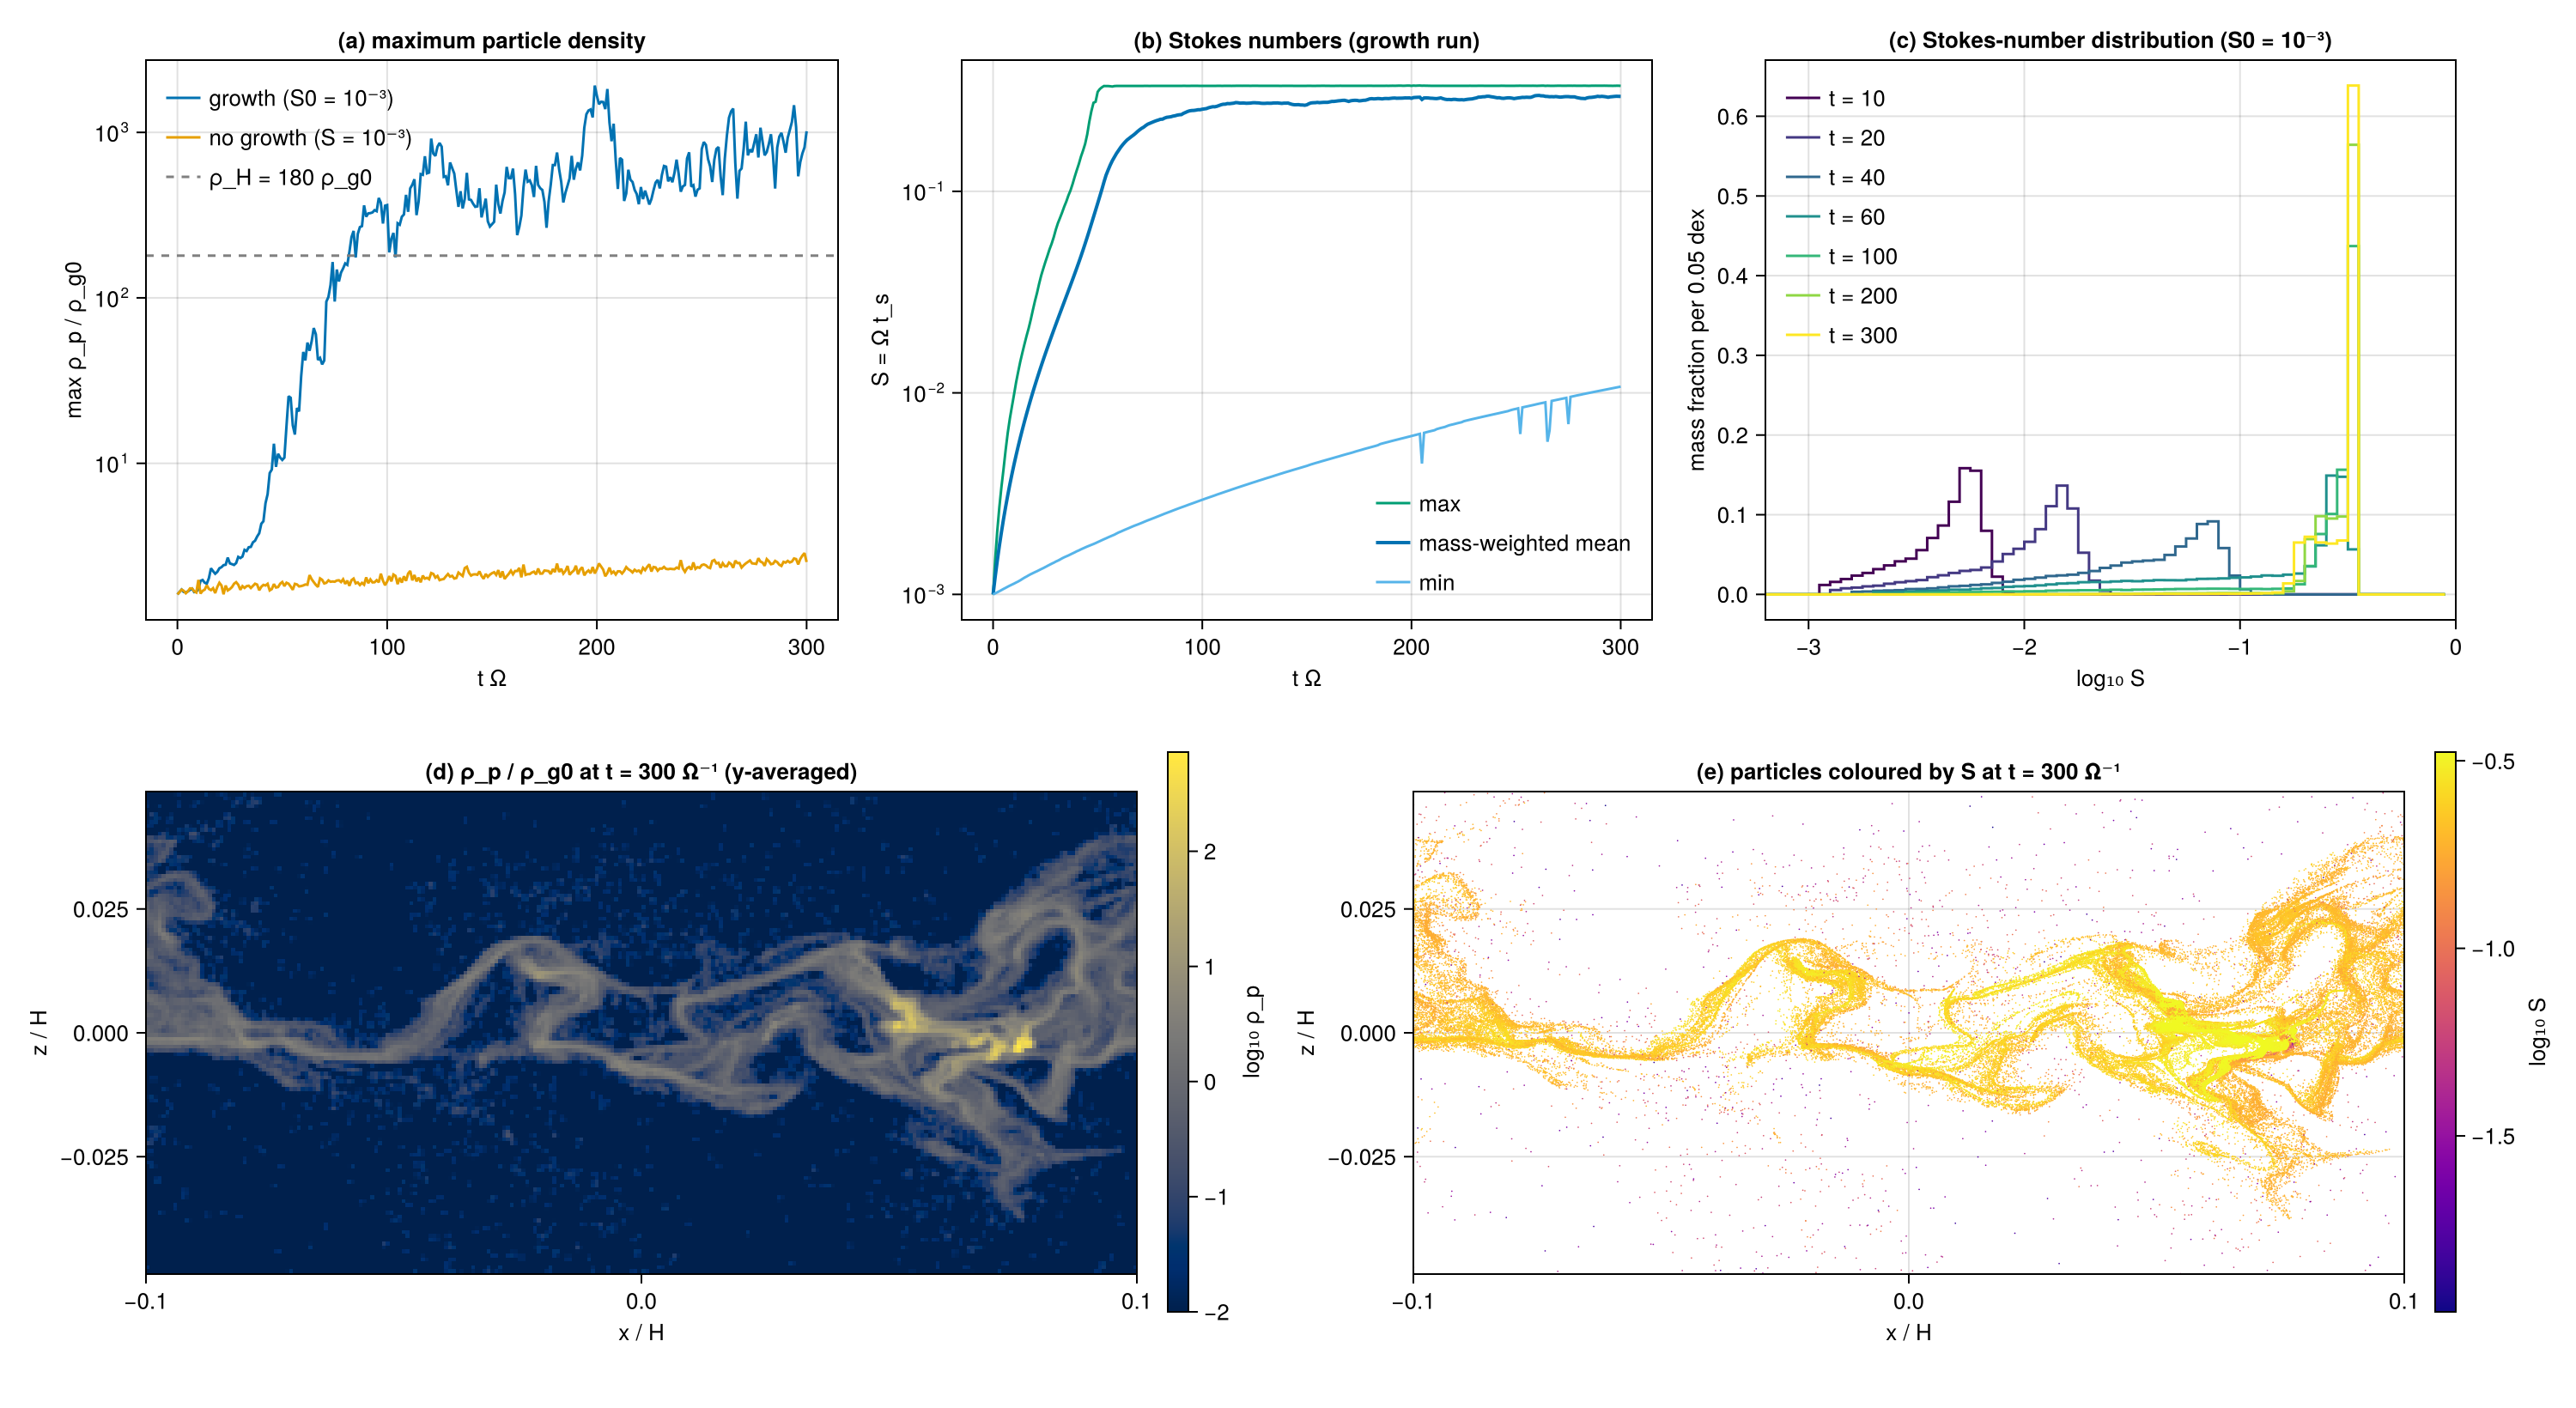
\includegraphics[width=\linewidth]{figures/dust_growth_r1_t300.png}
\caption{R1 at $1280/H$. (a) Maximum particle density of the growth run (blue) and the
no-growth control (orange), with the Hill density $180\rho_{g0}$; (b) Stokes-number
statistics of the growth run; (c) mass distribution of $\St$ at several times; (d)
$y$-averaged particle density and (e) particles coloured by $\St$ at
$t=300\,\Omega^{-1}$.}
\label{fig:r1}
\end{figure}

\paragraph{Data.} Run directories \file{/data/limjay/runs/si\_growth\_r1/\{fid,nogrowth\}}
on h-2 (0.89 and 0.86 GB); archived on October 20 as \code{<run>\_meta.tar} (histories,
logs, input, binary), \code{<run>\_data.tar} (restart, mesh and particle VTK files) and
\code{<run>.sha256} in \file{/data/limjay/archive\_dust\_growth} for transfer to Lou
(checksums verified; the tar contents add up byte for byte to the run directories). The figure is made by
\file{julia scripts/analysis/si\_growth\_r1\_fig.jl <fid dir> <nogrowth dir> <out.png>}
from the \code{phst} files, the particle VTK files at
$t=10, 20, 40, 60, 100, 200, 300$ and the dust density at $t=300$.

%=========================================================================================
\section{Notes from setting up}
\begin{itemize}
\item A new worktree starts with an empty \code{kokkos} submodule. The configured
  submodule URL is a local path, so it initialises without network access with
  \code{git -c protocol.file.allow=always submodule update --init kokkos}.
\item h-2 has no \code{rsync}; the source was copied with \code{tar} over \code{ssh}. A
  first copy with \code{--exclude './build*'} also dropped
  \file{kokkos/cmake/build\_env\_info.cmake} and \file{src/mesh/build\_tree.cpp} (bsdtar
  matches the pattern below the top level); the missing files were copied and the source
  list checked against \code{git ls-files}.
\end{itemize}

\end{document}
